\documentclass[twoside]{book}

% Packages required by doxygen
\usepackage{fixltx2e}
\usepackage{calc}
\usepackage{doxygen}
\usepackage[export]{adjustbox} % also loads graphicx
\usepackage{graphicx}
\usepackage[utf8]{inputenc}
\usepackage{makeidx}
\usepackage{multicol}
\usepackage{multirow}
\PassOptionsToPackage{warn}{textcomp}
\usepackage{textcomp}
\usepackage[nointegrals]{wasysym}
\usepackage[table]{xcolor}

% Font selection
\usepackage[T1]{fontenc}
\usepackage[scaled=.90]{helvet}
\usepackage{courier}
\usepackage{amssymb}
\usepackage{sectsty}
\renewcommand{\familydefault}{\sfdefault}
\allsectionsfont{%
  \fontseries{bc}\selectfont%
  \color{darkgray}%
}
\renewcommand{\DoxyLabelFont}{%
  \fontseries{bc}\selectfont%
  \color{darkgray}%
}
\newcommand{\+}{\discretionary{\mbox{\scriptsize$\hookleftarrow$}}{}{}}

% Page & text layout
\usepackage{geometry}
\geometry{%
  a4paper,%
  top=2.5cm,%
  bottom=2.5cm,%
  left=2.5cm,%
  right=2.5cm%
}
\tolerance=750
\hfuzz=15pt
\hbadness=750
\setlength{\emergencystretch}{15pt}
\setlength{\parindent}{0cm}
\setlength{\parskip}{3ex plus 2ex minus 2ex}
\makeatletter
\renewcommand{\paragraph}{%
  \@startsection{paragraph}{4}{0ex}{-1.0ex}{1.0ex}{%
    \normalfont\normalsize\bfseries\SS@parafont%
  }%
}
\renewcommand{\subparagraph}{%
  \@startsection{subparagraph}{5}{0ex}{-1.0ex}{1.0ex}{%
    \normalfont\normalsize\bfseries\SS@subparafont%
  }%
}
\makeatother

% Headers & footers
\usepackage{fancyhdr}
\pagestyle{fancyplain}
\fancyhead[LE]{\fancyplain{}{\bfseries\thepage}}
\fancyhead[CE]{\fancyplain{}{}}
\fancyhead[RE]{\fancyplain{}{\bfseries\leftmark}}
\fancyhead[LO]{\fancyplain{}{\bfseries\rightmark}}
\fancyhead[CO]{\fancyplain{}{}}
\fancyhead[RO]{\fancyplain{}{\bfseries\thepage}}
\fancyfoot[LE]{\fancyplain{}{}}
\fancyfoot[CE]{\fancyplain{}{}}
\fancyfoot[RE]{\fancyplain{}{\bfseries\scriptsize Generated by Doxygen }}
\fancyfoot[LO]{\fancyplain{}{\bfseries\scriptsize Generated by Doxygen }}
\fancyfoot[CO]{\fancyplain{}{}}
\fancyfoot[RO]{\fancyplain{}{}}
\renewcommand{\footrulewidth}{0.4pt}
\renewcommand{\chaptermark}[1]{%
  \markboth{#1}{}%
}
\renewcommand{\sectionmark}[1]{%
  \markright{\thesection\ #1}%
}

% Indices & bibliography
\usepackage{natbib}
\usepackage[titles]{tocloft}
\setcounter{tocdepth}{3}
\setcounter{secnumdepth}{5}
\makeindex

% Hyperlinks (required, but should be loaded last)
\usepackage{ifpdf}
\ifpdf
  \usepackage[pdftex,pagebackref=true]{hyperref}
\else
  \usepackage[ps2pdf,pagebackref=true]{hyperref}
\fi
\hypersetup{%
  colorlinks=true,%
  linkcolor=blue,%
  citecolor=blue,%
  unicode%
}

% Custom commands
\newcommand{\clearemptydoublepage}{%
  \newpage{\pagestyle{empty}\cleardoublepage}%
}

\usepackage{caption}
\captionsetup{labelsep=space,justification=centering,font={bf},singlelinecheck=off,skip=4pt,position=top}

%===== C O N T E N T S =====

\begin{document}

% Titlepage & ToC
\hypersetup{pageanchor=false,
             bookmarksnumbered=true,
             pdfencoding=unicode
            }
\pagenumbering{roman}
\begin{titlepage}
\vspace*{7cm}
\begin{center}%
{\Large My Project }\\
\vspace*{1cm}
{\large Generated by Doxygen 1.8.11}\\
\end{center}
\end{titlepage}
\clearemptydoublepage
\tableofcontents
\clearemptydoublepage
\pagenumbering{arabic}
\hypersetup{pageanchor=true}

%--- Begin generated contents ---
\chapter{Class Index}
\section{Class List}
Here are the classes, structs, unions and interfaces with brief descriptions\+:\begin{DoxyCompactList}
\item\contentsline{section}{\hyperlink{structnode}{node} }{\pageref{structnode}}{}
\item\contentsline{section}{\hyperlink{structnode1}{node1} }{\pageref{structnode1}}{}
\item\contentsline{section}{\hyperlink{structnode__info}{node\+\_\+info} }{\pageref{structnode__info}}{}
\end{DoxyCompactList}

\chapter{File Index}
\section{File List}
Here is a list of all files with brief descriptions\+:\begin{DoxyCompactList}
\item\contentsline{section}{\hyperlink{Lab1_8c}{Lab1.\+c} }{\pageref{Lab1_8c}}{}
\end{DoxyCompactList}

\chapter{Class Documentation}
\hypertarget{classDate}{}\section{Date Class Reference}
\label{classDate}\index{Date@{Date}}


{\ttfamily \#include $<$Date.\+h$>$}

\subsection*{Public Member Functions}
\begin{DoxyCompactItemize}
\item 
\hyperlink{classDate_a147bd9e8e7a33cc62c60f2ce3d46fbf5}{Date} (int y, int m, int d)
\item 
void \hyperlink{classDate_a4ed169cf9b2c9670083ac2f1e87729ff}{set\+Date} (int y, int m, int d)
\item 
int \hyperlink{classDate_acbe0df036d53e8ddcfa96523177bbd23}{get\+Year} () const 
\item 
int \hyperlink{classDate_a378143c24ab06d9dd38712fc515056dc}{get\+Month} () const 
\item 
int \hyperlink{classDate_a9114656893af6950f86e9438c9d01c77}{get\+Day} () const 
\item 
void \hyperlink{classDate_ae50d821702b1998f10487e6eee3f4785}{set\+Year} (int y)
\item 
void \hyperlink{classDate_ab137497d665577fb8a5e964eafd7dbfd}{set\+Month} (int m)
\item 
void \hyperlink{classDate_a785b3d8fbce101d565528b9032cea462}{set\+Day} (int d)
\item 
void \hyperlink{classDate_a7c3881597e07d4e1ccb50037eca79ec5}{print} () const 
\item 
\hyperlink{classDate}{Date} \& \hyperlink{classDate_af260b6e2ba7e7aa2fcca0d6bbafb3573}{next\+Day} ()
\item 
\hyperlink{classDate}{Date} \& \hyperlink{classDate_aa6ce7ce31fa0a127343f0626aefa40e0}{previous\+Day} ()
\item 
\hyperlink{classDate}{Date} \& \hyperlink{classDate_a708a38641ee9c2365a53090364f92fc0}{next\+Month} ()
\item 
\hyperlink{classDate}{Date} \& \hyperlink{classDate_a95307f1900d32b98caedb959988361f2}{previous\+Month} ()
\item 
\hyperlink{classDate}{Date} \& \hyperlink{classDate_a4835307418add39a9cbc4f2c6654246d}{next\+Year} ()
\item 
\hyperlink{classDate}{Date} \& \hyperlink{classDate_aa6fa73ef9aa2e87c72c567b26af9889b}{previous\+Year} ()
\end{DoxyCompactItemize}
\subsection*{Static Public Member Functions}
\begin{DoxyCompactItemize}
\item 
static bool \hyperlink{classDate_a208f91be271883b3225ca83a5ce4b5c6}{is\+Leap\+Year} (int y)
\item 
static bool \hyperlink{classDate_a0fda37dbf9ad83f6e1d1ecb2352f2de1}{is\+Valid\+Date} (int y, int m, int d)
\item 
static int \hyperlink{classDate_a16ea54d4178d24268ed3929b1a483bce}{get\+Day\+Of\+Week} (int y, int m, int d)
\end{DoxyCompactItemize}
\subsection*{Private Attributes}
\begin{DoxyCompactItemize}
\item 
int \hyperlink{classDate_a3eeced2ed56bc95d56782b9e738db8ea}{year}
\item 
int \hyperlink{classDate_a533843e07c6ac8d19fee9b16f5336ba2}{month}
\item 
int \hyperlink{classDate_a5b192adcabf2b2871e3f0b76c1ec1601}{day}
\end{DoxyCompactItemize}
\subsection*{Static Private Attributes}
\begin{DoxyCompactItemize}
\item 
static const string \hyperlink{classDate_a384a8a994b7f860051bc83e61a49a5f8}{S\+T\+R\+\_\+\+M\+O\+N\+T\+HS} \mbox{[}$\,$\mbox{]}
\item 
static const string \hyperlink{classDate_a9e9df675754c43945320ebbf20c90995}{S\+T\+R\+\_\+\+D\+A\+YS} \mbox{[}$\,$\mbox{]}
\item 
static const int \hyperlink{classDate_a2f9826c78c8945c8b584d1e19ea33ade}{D\+A\+Y\+S\+\_\+\+I\+N\+\_\+\+M\+O\+N\+T\+HS} \mbox{[}$\,$\mbox{]} = \{31, 28, 31, 30, 31, 30, 31, 31, 30, 31, 30, 31\}
\item 
static const int \hyperlink{classDate_a2c6e3f38e03c9de55218098acf40537f}{Y\+E\+A\+R\+\_\+\+M\+IN} = 1753
\item 
static const int \hyperlink{classDate_aded4c3bb2f76583cfc3da4f6932f3af1}{Y\+E\+A\+R\+\_\+\+M\+AX} = 9999
\end{DoxyCompactItemize}


\subsection{Constructor \& Destructor Documentation}
\index{Date@{Date}!Date@{Date}}
\index{Date@{Date}!Date@{Date}}
\subsubsection[{\texorpdfstring{Date(int y, int m, int d)}{Date(int y, int m, int d)}}]{\setlength{\rightskip}{0pt plus 5cm}Date\+::\+Date (
\begin{DoxyParamCaption}
\item[{int}]{y, }
\item[{int}]{m, }
\item[{int}]{d}
\end{DoxyParamCaption}
)}\hypertarget{classDate_a147bd9e8e7a33cc62c60f2ce3d46fbf5}{}\label{classDate_a147bd9e8e7a33cc62c60f2ce3d46fbf5}

\begin{DoxyCode}
59                               \{
60    \hyperlink{classDate_a4ed169cf9b2c9670083ac2f1e87729ff}{setDate}(y, m, d);
61 \}
\end{DoxyCode}


\subsection{Member Function Documentation}
\index{Date@{Date}!get\+Day@{get\+Day}}
\index{get\+Day@{get\+Day}!Date@{Date}}
\subsubsection[{\texorpdfstring{get\+Day() const }{getDay() const }}]{\setlength{\rightskip}{0pt plus 5cm}int Date\+::get\+Day (
\begin{DoxyParamCaption}
{}
\end{DoxyParamCaption}
) const}\hypertarget{classDate_a9114656893af6950f86e9438c9d01c77}{}\label{classDate_a9114656893af6950f86e9438c9d01c77}

\begin{DoxyCode}
94                        \{
95    \textcolor{keywordflow}{return} \hyperlink{classDate_a5b192adcabf2b2871e3f0b76c1ec1601}{day};
96 \}
\end{DoxyCode}
\index{Date@{Date}!get\+Day\+Of\+Week@{get\+Day\+Of\+Week}}
\index{get\+Day\+Of\+Week@{get\+Day\+Of\+Week}!Date@{Date}}
\subsubsection[{\texorpdfstring{get\+Day\+Of\+Week(int y, int m, int d)}{getDayOfWeek(int y, int m, int d)}}]{\setlength{\rightskip}{0pt plus 5cm}int Date\+::get\+Day\+Of\+Week (
\begin{DoxyParamCaption}
\item[{int}]{y, }
\item[{int}]{m, }
\item[{int}]{d}
\end{DoxyParamCaption}
)\hspace{0.3cm}{\ttfamily [static]}}\hypertarget{classDate_a16ea54d4178d24268ed3929b1a483bce}{}\label{classDate_a16ea54d4178d24268ed3929b1a483bce}

\begin{DoxyCode}
36                                           \{
37    \textcolor{keywordtype}{int} centuryTable[] = \{4, 2, 0, 6, 4, 2, 0, 6\}; \textcolor{comment}{// 17xx, 18xx, ...}
38    \textcolor{keywordtype}{int} MonthTable[] = \{0, 3, 3, 6, 1, 4, 6, 2, 5, 0, 3, 5\};
39    \textcolor{keywordtype}{int} MonthLeapYearTable[] = \{6, 2, 3, 6, 1, 4, 6, 2, 5, 0, 3, 5\};
40  
41    \textcolor{keywordtype}{int} century = y / 100;
42    \textcolor{keywordtype}{int} twoDigitYear = y % 100;
43    \textcolor{keywordtype}{int} centuryTableIndex = (century - 17) % 8;
44    \textcolor{comment}{// Date before 17xx are not valid, but needed to prevent negative index}
45    \textcolor{keywordflow}{if} (centuryTableIndex < 0) \{
46       centuryTableIndex += 8;
47    \}
48    \textcolor{keywordtype}{int} sum = centuryTable[centuryTableIndex] + twoDigitYear + twoDigitYear / 4;
49    \textcolor{keywordflow}{if} (\hyperlink{classDate_a208f91be271883b3225ca83a5ce4b5c6}{isLeapYear}(y)) \{
50       sum += MonthLeapYearTable[m-1];
51    \} \textcolor{keywordflow}{else} \{
52       sum += MonthTable[m-1];
53    \}
54    sum += d;
55    \textcolor{keywordflow}{return} sum % 7;
56 \}
\end{DoxyCode}
\index{Date@{Date}!get\+Month@{get\+Month}}
\index{get\+Month@{get\+Month}!Date@{Date}}
\subsubsection[{\texorpdfstring{get\+Month() const }{getMonth() const }}]{\setlength{\rightskip}{0pt plus 5cm}int Date\+::get\+Month (
\begin{DoxyParamCaption}
{}
\end{DoxyParamCaption}
) const}\hypertarget{classDate_a378143c24ab06d9dd38712fc515056dc}{}\label{classDate_a378143c24ab06d9dd38712fc515056dc}

\begin{DoxyCode}
82                          \{
83    \textcolor{keywordflow}{return} \hyperlink{classDate_a533843e07c6ac8d19fee9b16f5336ba2}{month};
84 \}
\end{DoxyCode}
\index{Date@{Date}!get\+Year@{get\+Year}}
\index{get\+Year@{get\+Year}!Date@{Date}}
\subsubsection[{\texorpdfstring{get\+Year() const }{getYear() const }}]{\setlength{\rightskip}{0pt plus 5cm}int Date\+::get\+Year (
\begin{DoxyParamCaption}
{}
\end{DoxyParamCaption}
) const}\hypertarget{classDate_acbe0df036d53e8ddcfa96523177bbd23}{}\label{classDate_acbe0df036d53e8ddcfa96523177bbd23}

\begin{DoxyCode}
70                         \{
71    \textcolor{keywordflow}{return} \hyperlink{classDate_a3eeced2ed56bc95d56782b9e738db8ea}{year};
72 \}
\end{DoxyCode}
\index{Date@{Date}!is\+Leap\+Year@{is\+Leap\+Year}}
\index{is\+Leap\+Year@{is\+Leap\+Year}!Date@{Date}}
\subsubsection[{\texorpdfstring{is\+Leap\+Year(int y)}{isLeapYear(int y)}}]{\setlength{\rightskip}{0pt plus 5cm}bool Date\+::is\+Leap\+Year (
\begin{DoxyParamCaption}
\item[{int}]{y}
\end{DoxyParamCaption}
)\hspace{0.3cm}{\ttfamily [static]}}\hypertarget{classDate_a208f91be271883b3225ca83a5ce4b5c6}{}\label{classDate_a208f91be271883b3225ca83a5ce4b5c6}

\begin{DoxyCode}
17                               \{
18    \textcolor{keywordflow}{return} ((\hyperlink{classDate_a3eeced2ed56bc95d56782b9e738db8ea}{year} % 4 == 0 && \hyperlink{classDate_a3eeced2ed56bc95d56782b9e738db8ea}{year} % 100 != 0) || (\hyperlink{classDate_a3eeced2ed56bc95d56782b9e738db8ea}{year} % 400 == 0));
19 \}
\end{DoxyCode}
\index{Date@{Date}!is\+Valid\+Date@{is\+Valid\+Date}}
\index{is\+Valid\+Date@{is\+Valid\+Date}!Date@{Date}}
\subsubsection[{\texorpdfstring{is\+Valid\+Date(int y, int m, int d)}{isValidDate(int y, int m, int d)}}]{\setlength{\rightskip}{0pt plus 5cm}bool Date\+::is\+Valid\+Date (
\begin{DoxyParamCaption}
\item[{int}]{y, }
\item[{int}]{m, }
\item[{int}]{d}
\end{DoxyParamCaption}
)\hspace{0.3cm}{\ttfamily [static]}}\hypertarget{classDate_a0fda37dbf9ad83f6e1d1ecb2352f2de1}{}\label{classDate_a0fda37dbf9ad83f6e1d1ecb2352f2de1}

\begin{DoxyCode}
22                                           \{
23    \textcolor{keywordflow}{if} (y >= \hyperlink{classDate_a2c6e3f38e03c9de55218098acf40537f}{YEAR\_MIN} && y <= YEAR\_MAX && m >= 1 && m <= 12) \{
24       \textcolor{keywordtype}{int} lastDayOfMonth = \hyperlink{classDate_a2f9826c78c8945c8b584d1e19ea33ade}{DAYS\_IN\_MONTHS}[m-1];
25       \textcolor{keywordflow}{if} (m == 2 && \hyperlink{classDate_a208f91be271883b3225ca83a5ce4b5c6}{isLeapYear}(y)) \{
26          lastDayOfMonth = 29;
27       \}
28       \textcolor{keywordflow}{return} (d >= 1 && d <= lastDayOfMonth);
29    \} \textcolor{keywordflow}{else} \{
30       \textcolor{keywordflow}{return} \textcolor{keyword}{false};
31    \}
32 \}
\end{DoxyCode}
\index{Date@{Date}!next\+Day@{next\+Day}}
\index{next\+Day@{next\+Day}!Date@{Date}}
\subsubsection[{\texorpdfstring{next\+Day()}{nextDay()}}]{\setlength{\rightskip}{0pt plus 5cm}{\bf Date} \& Date\+::next\+Day (
\begin{DoxyParamCaption}
{}
\end{DoxyParamCaption}
)}\hypertarget{classDate_af260b6e2ba7e7aa2fcca0d6bbafb3573}{}\label{classDate_af260b6e2ba7e7aa2fcca0d6bbafb3573}

\begin{DoxyCode}
118                     \{
119    \textcolor{keywordtype}{int} lastDayOfMonth = \hyperlink{classDate_a2f9826c78c8945c8b584d1e19ea33ade}{DAYS\_IN\_MONTHS}[\hyperlink{classDate_a533843e07c6ac8d19fee9b16f5336ba2}{month}-1];
120    \textcolor{keywordflow}{if} (\hyperlink{classDate_a533843e07c6ac8d19fee9b16f5336ba2}{month} == 2 && \hyperlink{classDate_a208f91be271883b3225ca83a5ce4b5c6}{isLeapYear}(\hyperlink{classDate_a3eeced2ed56bc95d56782b9e738db8ea}{year})) \{
121       lastDayOfMonth = 29;
122    \}
123  
124    \textcolor{comment}{// check day against the end of month}
125    \textcolor{keywordflow}{if} (++\hyperlink{classDate_a5b192adcabf2b2871e3f0b76c1ec1601}{day} > lastDayOfMonth) \{
126       \hyperlink{classDate_a5b192adcabf2b2871e3f0b76c1ec1601}{day} = 1;
127       \textcolor{keywordflow}{if} (++\hyperlink{classDate_a533843e07c6ac8d19fee9b16f5336ba2}{month} > 12) \{
128          \hyperlink{classDate_a533843e07c6ac8d19fee9b16f5336ba2}{month} = 1;
129          \textcolor{keywordflow}{if} (++\hyperlink{classDate_a3eeced2ed56bc95d56782b9e738db8ea}{year} > \hyperlink{classDate_aded4c3bb2f76583cfc3da4f6932f3af1}{YEAR\_MAX}) \{
130             \textcolor{keywordflow}{throw} out\_of\_range(\textcolor{stringliteral}{"Error: Next day is out of range!"});
131          \}
132       \}
133    \}
134    \textcolor{keywordflow}{return} *\textcolor{keyword}{this};
135 \}
\end{DoxyCode}
\index{Date@{Date}!next\+Month@{next\+Month}}
\index{next\+Month@{next\+Month}!Date@{Date}}
\subsubsection[{\texorpdfstring{next\+Month()}{nextMonth()}}]{\setlength{\rightskip}{0pt plus 5cm}{\bf Date} \& Date\+::next\+Month (
\begin{DoxyParamCaption}
{}
\end{DoxyParamCaption}
)}\hypertarget{classDate_a708a38641ee9c2365a53090364f92fc0}{}\label{classDate_a708a38641ee9c2365a53090364f92fc0}

\begin{DoxyCode}
158                       \{
159    \textcolor{keywordflow}{if} (++\hyperlink{classDate_a533843e07c6ac8d19fee9b16f5336ba2}{month} > 12) \{
160       \hyperlink{classDate_a533843e07c6ac8d19fee9b16f5336ba2}{month} = 1;
161       \textcolor{keywordflow}{if} (++\hyperlink{classDate_a3eeced2ed56bc95d56782b9e738db8ea}{year} > \hyperlink{classDate_aded4c3bb2f76583cfc3da4f6932f3af1}{YEAR\_MAX}) \{
162          \textcolor{keywordflow}{throw} out\_of\_range(\textcolor{stringliteral}{"Error: Next month is out of range!"});
163       \}
164    \}
165    \textcolor{comment}{// may need to adjust the last day of the month}
166    \textcolor{keywordtype}{int} lastDayOfMonth = \hyperlink{classDate_a2f9826c78c8945c8b584d1e19ea33ade}{DAYS\_IN\_MONTHS}[\hyperlink{classDate_a533843e07c6ac8d19fee9b16f5336ba2}{month}-1];
167    \textcolor{keywordflow}{if} (\hyperlink{classDate_a533843e07c6ac8d19fee9b16f5336ba2}{month} == 2 && \hyperlink{classDate_a208f91be271883b3225ca83a5ce4b5c6}{isLeapYear}(\hyperlink{classDate_a3eeced2ed56bc95d56782b9e738db8ea}{year})) \{
168       lastDayOfMonth = 29;
169    \}
170    \textcolor{keywordflow}{if} (\hyperlink{classDate_a5b192adcabf2b2871e3f0b76c1ec1601}{day} > lastDayOfMonth) \{
171       \hyperlink{classDate_a5b192adcabf2b2871e3f0b76c1ec1601}{day} = lastDayOfMonth;
172    \}
173    \textcolor{keywordflow}{return} *\textcolor{keyword}{this};
174 \}
\end{DoxyCode}
\index{Date@{Date}!next\+Year@{next\+Year}}
\index{next\+Year@{next\+Year}!Date@{Date}}
\subsubsection[{\texorpdfstring{next\+Year()}{nextYear()}}]{\setlength{\rightskip}{0pt plus 5cm}{\bf Date} \& Date\+::next\+Year (
\begin{DoxyParamCaption}
{}
\end{DoxyParamCaption}
)}\hypertarget{classDate_a4835307418add39a9cbc4f2c6654246d}{}\label{classDate_a4835307418add39a9cbc4f2c6654246d}

\begin{DoxyCode}
196                      \{
197    \textcolor{keywordflow}{if} (++\hyperlink{classDate_a3eeced2ed56bc95d56782b9e738db8ea}{year} > \hyperlink{classDate_aded4c3bb2f76583cfc3da4f6932f3af1}{YEAR\_MAX}) \{
198       \textcolor{keywordflow}{throw} out\_of\_range(\textcolor{stringliteral}{"Error: Next year is out of range!"});
199    \}
200    \textcolor{comment}{// may need to adjust the last day of the month for leap year (29 Feb)}
201    \textcolor{comment}{//  to non-leap year (28 Feb)}
202    \textcolor{keywordflow}{if} (\hyperlink{classDate_a533843e07c6ac8d19fee9b16f5336ba2}{month} == 2 && \hyperlink{classDate_a5b192adcabf2b2871e3f0b76c1ec1601}{day} == 29 && !\hyperlink{classDate_a208f91be271883b3225ca83a5ce4b5c6}{isLeapYear}(\hyperlink{classDate_a3eeced2ed56bc95d56782b9e738db8ea}{year})) \{
203       \hyperlink{classDate_a5b192adcabf2b2871e3f0b76c1ec1601}{day} = 28;
204    \}
205    \textcolor{keywordflow}{return} *\textcolor{keyword}{this};
206 \}
\end{DoxyCode}
\index{Date@{Date}!previous\+Day@{previous\+Day}}
\index{previous\+Day@{previous\+Day}!Date@{Date}}
\subsubsection[{\texorpdfstring{previous\+Day()}{previousDay()}}]{\setlength{\rightskip}{0pt plus 5cm}{\bf Date} \& Date\+::previous\+Day (
\begin{DoxyParamCaption}
{}
\end{DoxyParamCaption}
)}\hypertarget{classDate_aa6ce7ce31fa0a127343f0626aefa40e0}{}\label{classDate_aa6ce7ce31fa0a127343f0626aefa40e0}

\begin{DoxyCode}
138                         \{
139    \textcolor{keywordtype}{int} lastDayOfMonth = \hyperlink{classDate_a2f9826c78c8945c8b584d1e19ea33ade}{DAYS\_IN\_MONTHS}[\hyperlink{classDate_a533843e07c6ac8d19fee9b16f5336ba2}{month}-1];
140    \textcolor{keywordflow}{if} (\hyperlink{classDate_a533843e07c6ac8d19fee9b16f5336ba2}{month} == 2 && \hyperlink{classDate_a208f91be271883b3225ca83a5ce4b5c6}{isLeapYear}(\hyperlink{classDate_a3eeced2ed56bc95d56782b9e738db8ea}{year})) \{
141       lastDayOfMonth = 29;
142    \}
143  
144    \textcolor{comment}{// check day against the end of month}
145    \textcolor{keywordflow}{if} (--\hyperlink{classDate_a5b192adcabf2b2871e3f0b76c1ec1601}{day} < 1) \{
146       \hyperlink{classDate_a5b192adcabf2b2871e3f0b76c1ec1601}{day} = lastDayOfMonth;
147       \textcolor{keywordflow}{if} (--\hyperlink{classDate_a533843e07c6ac8d19fee9b16f5336ba2}{month} < 1) \{
148          \hyperlink{classDate_a533843e07c6ac8d19fee9b16f5336ba2}{month} = 12;
149          \textcolor{keywordflow}{if} (--\hyperlink{classDate_a3eeced2ed56bc95d56782b9e738db8ea}{year} < \hyperlink{classDate_a2c6e3f38e03c9de55218098acf40537f}{YEAR\_MIN}) \{
150             \textcolor{keywordflow}{throw} out\_of\_range(\textcolor{stringliteral}{"Error: Previous day is out of range!"});
151          \}
152       \}
153    \}
154    \textcolor{keywordflow}{return} *\textcolor{keyword}{this};
155 \}
\end{DoxyCode}
\index{Date@{Date}!previous\+Month@{previous\+Month}}
\index{previous\+Month@{previous\+Month}!Date@{Date}}
\subsubsection[{\texorpdfstring{previous\+Month()}{previousMonth()}}]{\setlength{\rightskip}{0pt plus 5cm}{\bf Date} \& Date\+::previous\+Month (
\begin{DoxyParamCaption}
{}
\end{DoxyParamCaption}
)}\hypertarget{classDate_a95307f1900d32b98caedb959988361f2}{}\label{classDate_a95307f1900d32b98caedb959988361f2}

\begin{DoxyCode}
177                           \{
178    \textcolor{keywordflow}{if} (--\hyperlink{classDate_a533843e07c6ac8d19fee9b16f5336ba2}{month} < 1) \{
179       \hyperlink{classDate_a533843e07c6ac8d19fee9b16f5336ba2}{month} = 12;
180       \textcolor{keywordflow}{if} (--\hyperlink{classDate_a3eeced2ed56bc95d56782b9e738db8ea}{year} < \hyperlink{classDate_a2c6e3f38e03c9de55218098acf40537f}{YEAR\_MIN}) \{
181          \textcolor{keywordflow}{throw} out\_of\_range(\textcolor{stringliteral}{"Error: Previous month is out of range!"});
182       \}
183    \}
184    \textcolor{comment}{// may need to adjust the last day of the month}
185    \textcolor{keywordtype}{int} lastDayOfMonth = \hyperlink{classDate_a2f9826c78c8945c8b584d1e19ea33ade}{DAYS\_IN\_MONTHS}[\hyperlink{classDate_a533843e07c6ac8d19fee9b16f5336ba2}{month}-1];
186    \textcolor{keywordflow}{if} (\hyperlink{classDate_a533843e07c6ac8d19fee9b16f5336ba2}{month} == 2 && \hyperlink{classDate_a208f91be271883b3225ca83a5ce4b5c6}{isLeapYear}(\hyperlink{classDate_a3eeced2ed56bc95d56782b9e738db8ea}{year})) \{
187       lastDayOfMonth = 29;
188    \}
189    \textcolor{keywordflow}{if} (\hyperlink{classDate_a5b192adcabf2b2871e3f0b76c1ec1601}{day} > lastDayOfMonth) \{
190       \hyperlink{classDate_a5b192adcabf2b2871e3f0b76c1ec1601}{day} = lastDayOfMonth;
191    \}
192    \textcolor{keywordflow}{return} *\textcolor{keyword}{this};
193 \}
\end{DoxyCode}
\index{Date@{Date}!previous\+Year@{previous\+Year}}
\index{previous\+Year@{previous\+Year}!Date@{Date}}
\subsubsection[{\texorpdfstring{previous\+Year()}{previousYear()}}]{\setlength{\rightskip}{0pt plus 5cm}{\bf Date} \& Date\+::previous\+Year (
\begin{DoxyParamCaption}
{}
\end{DoxyParamCaption}
)}\hypertarget{classDate_aa6fa73ef9aa2e87c72c567b26af9889b}{}\label{classDate_aa6fa73ef9aa2e87c72c567b26af9889b}

\begin{DoxyCode}
209                          \{
210    \textcolor{keywordflow}{if} (--\hyperlink{classDate_a3eeced2ed56bc95d56782b9e738db8ea}{year} < \hyperlink{classDate_a2c6e3f38e03c9de55218098acf40537f}{YEAR\_MIN}) \{
211       \textcolor{keywordflow}{throw} out\_of\_range(\textcolor{stringliteral}{"Error: Previous year is out of range!"});
212    \}
213    \textcolor{comment}{// may need to adjust the last day of the month for leap year (29 Feb)}
214    \textcolor{comment}{//  to non-leap year (28 Feb)}
215    \textcolor{keywordflow}{if} (\hyperlink{classDate_a533843e07c6ac8d19fee9b16f5336ba2}{month} == 2 && \hyperlink{classDate_a5b192adcabf2b2871e3f0b76c1ec1601}{day} == 29 && !\hyperlink{classDate_a208f91be271883b3225ca83a5ce4b5c6}{isLeapYear}(\hyperlink{classDate_a3eeced2ed56bc95d56782b9e738db8ea}{year})) \{
216       \hyperlink{classDate_a5b192adcabf2b2871e3f0b76c1ec1601}{day} = 28;
217    \}
218    \textcolor{keywordflow}{return} *\textcolor{keyword}{this};
219 \}\end{DoxyCode}
\index{Date@{Date}!print@{print}}
\index{print@{print}!Date@{Date}}
\subsubsection[{\texorpdfstring{print() const }{print() const }}]{\setlength{\rightskip}{0pt plus 5cm}void Date\+::print (
\begin{DoxyParamCaption}
{}
\end{DoxyParamCaption}
) const}\hypertarget{classDate_a7c3881597e07d4e1ccb50037eca79ec5}{}\label{classDate_a7c3881597e07d4e1ccb50037eca79ec5}

\begin{DoxyCode}
112                        \{
113    cout << \hyperlink{classDate_a9e9df675754c43945320ebbf20c90995}{STR\_DAYS}[\hyperlink{classDate_a16ea54d4178d24268ed3929b1a483bce}{getDayOfWeek}(\hyperlink{classDate_a3eeced2ed56bc95d56782b9e738db8ea}{year}, \hyperlink{classDate_a533843e07c6ac8d19fee9b16f5336ba2}{month}, \hyperlink{classDate_a5b192adcabf2b2871e3f0b76c1ec1601}{day})] << \textcolor{stringliteral}{", "}
114         << \hyperlink{classDate_a5b192adcabf2b2871e3f0b76c1ec1601}{day} << \textcolor{stringliteral}{" "} << \hyperlink{classDate_a384a8a994b7f860051bc83e61a49a5f8}{STR\_MONTHS}[\hyperlink{classDate_a533843e07c6ac8d19fee9b16f5336ba2}{month}-1] << \textcolor{stringliteral}{" "} << \hyperlink{classDate_a3eeced2ed56bc95d56782b9e738db8ea}{year} << endl;
115 \}
\end{DoxyCode}
\index{Date@{Date}!set\+Date@{set\+Date}}
\index{set\+Date@{set\+Date}!Date@{Date}}
\subsubsection[{\texorpdfstring{set\+Date(int y, int m, int d)}{setDate(int y, int m, int d)}}]{\setlength{\rightskip}{0pt plus 5cm}void Date\+::set\+Date (
\begin{DoxyParamCaption}
\item[{int}]{y, }
\item[{int}]{m, }
\item[{int}]{d}
\end{DoxyParamCaption}
)}\hypertarget{classDate_a4ed169cf9b2c9670083ac2f1e87729ff}{}\label{classDate_a4ed169cf9b2c9670083ac2f1e87729ff}

\begin{DoxyCode}
64                                       \{
65    \hyperlink{classDate_ae50d821702b1998f10487e6eee3f4785}{setYear}(y);
66    \hyperlink{classDate_ab137497d665577fb8a5e964eafd7dbfd}{setMonth}(m);
67    \hyperlink{classDate_a785b3d8fbce101d565528b9032cea462}{setDay}(d); \textcolor{comment}{// need to set the day after year and month}
68 \}
\end{DoxyCode}
\index{Date@{Date}!set\+Day@{set\+Day}}
\index{set\+Day@{set\+Day}!Date@{Date}}
\subsubsection[{\texorpdfstring{set\+Day(int d)}{setDay(int d)}}]{\setlength{\rightskip}{0pt plus 5cm}void Date\+::set\+Day (
\begin{DoxyParamCaption}
\item[{int}]{d}
\end{DoxyParamCaption}
)}\hypertarget{classDate_a785b3d8fbce101d565528b9032cea462}{}\label{classDate_a785b3d8fbce101d565528b9032cea462}

\begin{DoxyCode}
99                        \{
100    \textcolor{keywordtype}{int} lastDayOfMonth = \hyperlink{classDate_a2f9826c78c8945c8b584d1e19ea33ade}{DAYS\_IN\_MONTHS}[\hyperlink{classDate_a533843e07c6ac8d19fee9b16f5336ba2}{month}-1];
101    \textcolor{keywordflow}{if} (\hyperlink{classDate_a533843e07c6ac8d19fee9b16f5336ba2}{month} == 2 && \hyperlink{classDate_a208f91be271883b3225ca83a5ce4b5c6}{isLeapYear}(\hyperlink{classDate_a3eeced2ed56bc95d56782b9e738db8ea}{year})) \{
102       lastDayOfMonth = 29;
103    \}
104    \textcolor{keywordflow}{if} (d >= 1 && d <= lastDayOfMonth) \{
105       \hyperlink{classDate_a5b192adcabf2b2871e3f0b76c1ec1601}{day} = d;
106    \} \textcolor{keywordflow}{else} \{
107       \textcolor{keywordflow}{throw} invalid\_argument(\textcolor{stringliteral}{"Error: Invalid day (1-28|29|30|31)!"});
108    \}
109 \}
\end{DoxyCode}
\index{Date@{Date}!set\+Month@{set\+Month}}
\index{set\+Month@{set\+Month}!Date@{Date}}
\subsubsection[{\texorpdfstring{set\+Month(int m)}{setMonth(int m)}}]{\setlength{\rightskip}{0pt plus 5cm}void Date\+::set\+Month (
\begin{DoxyParamCaption}
\item[{int}]{m}
\end{DoxyParamCaption}
)}\hypertarget{classDate_ab137497d665577fb8a5e964eafd7dbfd}{}\label{classDate_ab137497d665577fb8a5e964eafd7dbfd}

\begin{DoxyCode}
86                          \{
87    \textcolor{keywordflow}{if} (m >= 1 && m <= 12) \{
88       \hyperlink{classDate_a533843e07c6ac8d19fee9b16f5336ba2}{month} = m;
89    \} \textcolor{keywordflow}{else} \{
90       \textcolor{keywordflow}{throw} invalid\_argument(\textcolor{stringliteral}{"Error: Invalid month (1-12)!"});
91    \}
92 \}
\end{DoxyCode}
\index{Date@{Date}!set\+Year@{set\+Year}}
\index{set\+Year@{set\+Year}!Date@{Date}}
\subsubsection[{\texorpdfstring{set\+Year(int y)}{setYear(int y)}}]{\setlength{\rightskip}{0pt plus 5cm}void Date\+::set\+Year (
\begin{DoxyParamCaption}
\item[{int}]{y}
\end{DoxyParamCaption}
)}\hypertarget{classDate_ae50d821702b1998f10487e6eee3f4785}{}\label{classDate_ae50d821702b1998f10487e6eee3f4785}

\begin{DoxyCode}
74                         \{
75    \textcolor{keywordflow}{if} (y >= \hyperlink{classDate_a2c6e3f38e03c9de55218098acf40537f}{YEAR\_MIN} && y <= \hyperlink{classDate_aded4c3bb2f76583cfc3da4f6932f3af1}{YEAR\_MAX}) \{
76       \hyperlink{classDate_a3eeced2ed56bc95d56782b9e738db8ea}{year} = y;
77    \} \textcolor{keywordflow}{else} \{
78       \textcolor{keywordflow}{throw} invalid\_argument(\textcolor{stringliteral}{"Error: Invalid year (1753-9999)!"});
79    \}
80 \}
\end{DoxyCode}


\subsection{Member Data Documentation}
\index{Date@{Date}!day@{day}}
\index{day@{day}!Date@{Date}}
\subsubsection[{\texorpdfstring{day}{day}}]{\setlength{\rightskip}{0pt plus 5cm}int Date\+::day\hspace{0.3cm}{\ttfamily [private]}}\hypertarget{classDate_a5b192adcabf2b2871e3f0b76c1ec1601}{}\label{classDate_a5b192adcabf2b2871e3f0b76c1ec1601}
\index{Date@{Date}!D\+A\+Y\+S\+\_\+\+I\+N\+\_\+\+M\+O\+N\+T\+HS@{D\+A\+Y\+S\+\_\+\+I\+N\+\_\+\+M\+O\+N\+T\+HS}}
\index{D\+A\+Y\+S\+\_\+\+I\+N\+\_\+\+M\+O\+N\+T\+HS@{D\+A\+Y\+S\+\_\+\+I\+N\+\_\+\+M\+O\+N\+T\+HS}!Date@{Date}}
\subsubsection[{\texorpdfstring{D\+A\+Y\+S\+\_\+\+I\+N\+\_\+\+M\+O\+N\+T\+HS}{DAYS_IN_MONTHS}}]{\setlength{\rightskip}{0pt plus 5cm}const int Date\+::\+D\+A\+Y\+S\+\_\+\+I\+N\+\_\+\+M\+O\+N\+T\+HS = \{31, 28, 31, 30, 31, 30, 31, 31, 30, 31, 30, 31\}\hspace{0.3cm}{\ttfamily [static]}, {\ttfamily [private]}}\hypertarget{classDate_a2f9826c78c8945c8b584d1e19ea33ade}{}\label{classDate_a2f9826c78c8945c8b584d1e19ea33ade}
\index{Date@{Date}!month@{month}}
\index{month@{month}!Date@{Date}}
\subsubsection[{\texorpdfstring{month}{month}}]{\setlength{\rightskip}{0pt plus 5cm}int Date\+::month\hspace{0.3cm}{\ttfamily [private]}}\hypertarget{classDate_a533843e07c6ac8d19fee9b16f5336ba2}{}\label{classDate_a533843e07c6ac8d19fee9b16f5336ba2}
\index{Date@{Date}!S\+T\+R\+\_\+\+D\+A\+YS@{S\+T\+R\+\_\+\+D\+A\+YS}}
\index{S\+T\+R\+\_\+\+D\+A\+YS@{S\+T\+R\+\_\+\+D\+A\+YS}!Date@{Date}}
\subsubsection[{\texorpdfstring{S\+T\+R\+\_\+\+D\+A\+YS}{STR_DAYS}}]{\setlength{\rightskip}{0pt plus 5cm}const string Date\+::\+S\+T\+R\+\_\+\+D\+A\+YS\hspace{0.3cm}{\ttfamily [static]}, {\ttfamily [private]}}\hypertarget{classDate_a9e9df675754c43945320ebbf20c90995}{}\label{classDate_a9e9df675754c43945320ebbf20c90995}
{\bfseries Initial value\+:}
\begin{DoxyCode}
= \{\textcolor{stringliteral}{"Sunday"}, \textcolor{stringliteral}{"Monday"}, \textcolor{stringliteral}{"Tuesday"}, \textcolor{stringliteral}{"Wednesday"},
                                 \textcolor{stringliteral}{"Thursday"}, \textcolor{stringliteral}{"Friday"}, \textcolor{stringliteral}{"Saturday"}\}
\end{DoxyCode}
\index{Date@{Date}!S\+T\+R\+\_\+\+M\+O\+N\+T\+HS@{S\+T\+R\+\_\+\+M\+O\+N\+T\+HS}}
\index{S\+T\+R\+\_\+\+M\+O\+N\+T\+HS@{S\+T\+R\+\_\+\+M\+O\+N\+T\+HS}!Date@{Date}}
\subsubsection[{\texorpdfstring{S\+T\+R\+\_\+\+M\+O\+N\+T\+HS}{STR_MONTHS}}]{\setlength{\rightskip}{0pt plus 5cm}const string Date\+::\+S\+T\+R\+\_\+\+M\+O\+N\+T\+HS\hspace{0.3cm}{\ttfamily [static]}, {\ttfamily [private]}}\hypertarget{classDate_a384a8a994b7f860051bc83e61a49a5f8}{}\label{classDate_a384a8a994b7f860051bc83e61a49a5f8}
{\bfseries Initial value\+:}
\begin{DoxyCode}
= \{\textcolor{stringliteral}{"Jan"}, \textcolor{stringliteral}{"Feb"}, \textcolor{stringliteral}{"Mar"}, \textcolor{stringliteral}{"Apr"}, \textcolor{stringliteral}{"May"}, \textcolor{stringliteral}{"Jun"},
                                   \textcolor{stringliteral}{"Jul"}, \textcolor{stringliteral}{"Aug"}, \textcolor{stringliteral}{"Sep"}, \textcolor{stringliteral}{"Oct"}, \textcolor{stringliteral}{"Nov"}, \textcolor{stringliteral}{"Dec"}\}
\end{DoxyCode}
\index{Date@{Date}!year@{year}}
\index{year@{year}!Date@{Date}}
\subsubsection[{\texorpdfstring{year}{year}}]{\setlength{\rightskip}{0pt plus 5cm}int Date\+::year\hspace{0.3cm}{\ttfamily [private]}}\hypertarget{classDate_a3eeced2ed56bc95d56782b9e738db8ea}{}\label{classDate_a3eeced2ed56bc95d56782b9e738db8ea}
\index{Date@{Date}!Y\+E\+A\+R\+\_\+\+M\+AX@{Y\+E\+A\+R\+\_\+\+M\+AX}}
\index{Y\+E\+A\+R\+\_\+\+M\+AX@{Y\+E\+A\+R\+\_\+\+M\+AX}!Date@{Date}}
\subsubsection[{\texorpdfstring{Y\+E\+A\+R\+\_\+\+M\+AX}{YEAR_MAX}}]{\setlength{\rightskip}{0pt plus 5cm}const int Date\+::\+Y\+E\+A\+R\+\_\+\+M\+AX = 9999\hspace{0.3cm}{\ttfamily [static]}, {\ttfamily [private]}}\hypertarget{classDate_aded4c3bb2f76583cfc3da4f6932f3af1}{}\label{classDate_aded4c3bb2f76583cfc3da4f6932f3af1}
\index{Date@{Date}!Y\+E\+A\+R\+\_\+\+M\+IN@{Y\+E\+A\+R\+\_\+\+M\+IN}}
\index{Y\+E\+A\+R\+\_\+\+M\+IN@{Y\+E\+A\+R\+\_\+\+M\+IN}!Date@{Date}}
\subsubsection[{\texorpdfstring{Y\+E\+A\+R\+\_\+\+M\+IN}{YEAR_MIN}}]{\setlength{\rightskip}{0pt plus 5cm}const int Date\+::\+Y\+E\+A\+R\+\_\+\+M\+IN = 1753\hspace{0.3cm}{\ttfamily [static]}, {\ttfamily [private]}}\hypertarget{classDate_a2c6e3f38e03c9de55218098acf40537f}{}\label{classDate_a2c6e3f38e03c9de55218098acf40537f}


The documentation for this class was generated from the following files\+:\begin{DoxyCompactItemize}
\item 
\hyperlink{Date_8h}{Date.\+h}\item 
\hyperlink{Date_8cpp}{Date.\+cpp}\end{DoxyCompactItemize}

\chapter{File Documentation}
\hypertarget{Date_8cpp}{}\section{Date.\+cpp File Reference}
\label{Date_8cpp}\index{Date.\+cpp@{Date.\+cpp}}
{\ttfamily \#include $<$iostream$>$}\\*
{\ttfamily \#include $<$stdexcept$>$}\\*
{\ttfamily \#include \char`\"{}Date.\+h\char`\"{}}\\*
Include dependency graph for Date.\+cpp\+:
\nopagebreak
\begin{figure}[H]
\begin{center}
\leavevmode
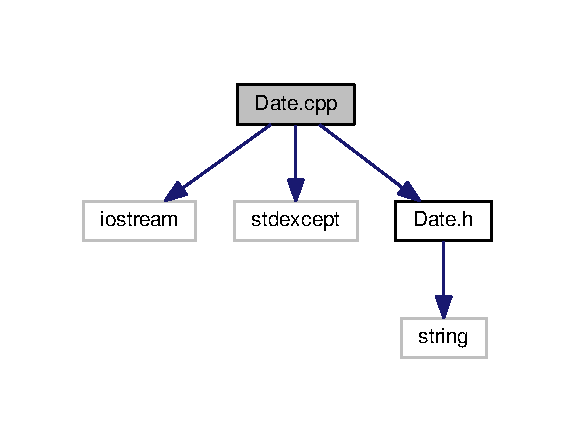
\includegraphics[width=276pt]{Date_8cpp__incl}
\end{center}
\end{figure}

\hypertarget{Date_8h}{}\section{Date.\+h File Reference}
\label{Date_8h}\index{Date.\+h@{Date.\+h}}
{\ttfamily \#include $<$string$>$}\\*
Include dependency graph for Date.\+h\+:
\nopagebreak
\begin{figure}[H]
\begin{center}
\leavevmode
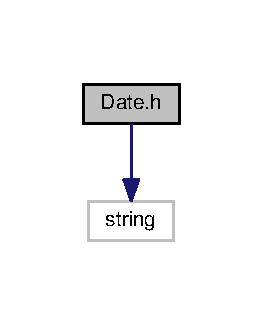
\includegraphics[width=126pt]{Date_8h__incl}
\end{center}
\end{figure}
This graph shows which files directly or indirectly include this file\+:
\nopagebreak
\begin{figure}[H]
\begin{center}
\leavevmode
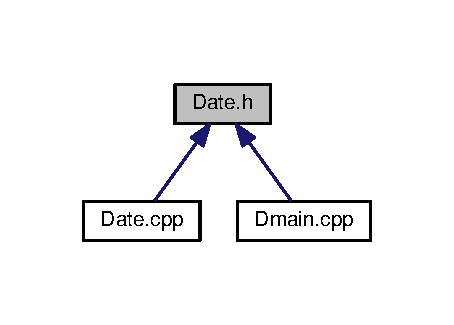
\includegraphics[width=218pt]{Date_8h__dep__incl}
\end{center}
\end{figure}
\subsection*{Classes}
\begin{DoxyCompactItemize}
\item 
class \hyperlink{classDate}{Date}
\end{DoxyCompactItemize}

\hypertarget{Dmain_8cpp}{}\section{Dmain.\+cpp File Reference}
\label{Dmain_8cpp}\index{Dmain.\+cpp@{Dmain.\+cpp}}
{\ttfamily \#include $<$iostream$>$}\\*
{\ttfamily \#include $<$stdexcept$>$}\\*
{\ttfamily \#include \char`\"{}Date.\+h\char`\"{}}\\*
Include dependency graph for Dmain.\+cpp\+:
\nopagebreak
\begin{figure}[H]
\begin{center}
\leavevmode
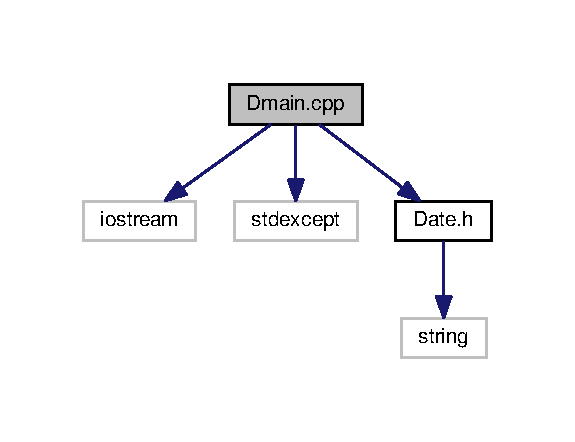
\includegraphics[width=276pt]{Dmain_8cpp__incl}
\end{center}
\end{figure}
\subsection*{Functions}
\begin{DoxyCompactItemize}
\item 
int \hyperlink{Dmain_8cpp_ae66f6b31b5ad750f1fe042a706a4e3d4}{main} ()
\end{DoxyCompactItemize}


\subsection{Function Documentation}
\index{Dmain.\+cpp@{Dmain.\+cpp}!main@{main}}
\index{main@{main}!Dmain.\+cpp@{Dmain.\+cpp}}
\subsubsection[{\texorpdfstring{main()}{main()}}]{\setlength{\rightskip}{0pt plus 5cm}int main (
\begin{DoxyParamCaption}
{}
\end{DoxyParamCaption}
)}\hypertarget{Dmain_8cpp_ae66f6b31b5ad750f1fe042a706a4e3d4}{}\label{Dmain_8cpp_ae66f6b31b5ad750f1fe042a706a4e3d4}

\begin{DoxyCode}
6            \{
7    \hyperlink{classDate}{Date} d1(2012, 1, 1);
8    d1.print();  \textcolor{comment}{// Sunday, 1 Jan 2012}
9    d1.nextDay().print();  \textcolor{comment}{// Monday, 2 Jan 2012}
10    d1.print();  \textcolor{comment}{// Monday, 2 Jan 2012}
11  
12    d1.setDate(2012, 1, 31);
13    d1.print();  \textcolor{comment}{// Tuesday, 31 Jan 2012}
14    d1.nextDay().print();  \textcolor{comment}{// Wednesday, 1 Feb 2012}
15  
16    d1.setDate(2012, 2, 28);
17    d1.print();  \textcolor{comment}{// Tuesday, 28 Feb 2012}
18    d1.nextDay().print();  \textcolor{comment}{// Wednesday, 29 Feb 2012}
19  
20    d1.setDate(2012, 12, 31);
21    d1.print();  \textcolor{comment}{// Monday, 31 Dec 2012}
22    d1.nextDay().print();  \textcolor{comment}{// Tuesday, 1 Jan 2013}
23  
24 \textcolor{comment}{//   Date d2(2011, 2, 29);  // abrupt termination!}
25 \textcolor{comment}{//   d2.print();}
26  
27    \textcolor{keywordflow}{try} \{  \textcolor{comment}{// graceful handling of exception}
28       \hyperlink{classDate}{Date} d3(2011, 2, 29);
29       d3.print();
30    \} \textcolor{keywordflow}{catch} (invalid\_argument &ex) \{
31       cout << ex.what() << endl;  \textcolor{comment}{// Error: Invalid day (1-28|29|30|31)!}
32    \}
33    cout << \textcolor{stringliteral}{"Next Statement after try-catch"} << endl;
34  
35    \textcolor{keywordflow}{try} \{  \textcolor{comment}{// graceful handling of exception}
36       \hyperlink{classDate}{Date} d4(9999, 12, 30);
37       d4.nextDay().print(); \textcolor{comment}{// Friday, 31 Dec 9999}
38       d4.nextDay();
39       d4.print();
40    \} \textcolor{keywordflow}{catch} (out\_of\_range &ex) \{
41       cout << ex.what() << endl;  \textcolor{comment}{// Error: Next day is outside the valid range!}
42    \}
43  
44    \hyperlink{classDate}{Date} d5(2012, 1, 1);
45    d5.previousDay().print();  \textcolor{comment}{// Saturday, 31 Dec 2011}
46  
47    \hyperlink{classDate}{Date} d6(2012, 3, 31);
48    d6.nextMonth().print();  \textcolor{comment}{// Monday, 30 Apr 2012}
49  
50    \hyperlink{classDate}{Date} d7(2012, 3, 31);
51    d7.previousMonth().print();  \textcolor{comment}{// Wednesday, 29 Feb 2012}
52  
53    \hyperlink{classDate}{Date} d8(2012, 2, 29);
54    d8.nextYear().print(); \textcolor{comment}{// Thursday, 28 Feb 2013}
55  
56    \hyperlink{classDate}{Date} d9(2012, 2, 29);
57    d9.previousYear().print();  \textcolor{comment}{// Monday, 28 Feb 2011}
58 \}\end{DoxyCode}


Here is the call graph for this function\+:
\nopagebreak
\begin{figure}[H]
\begin{center}
\leavevmode
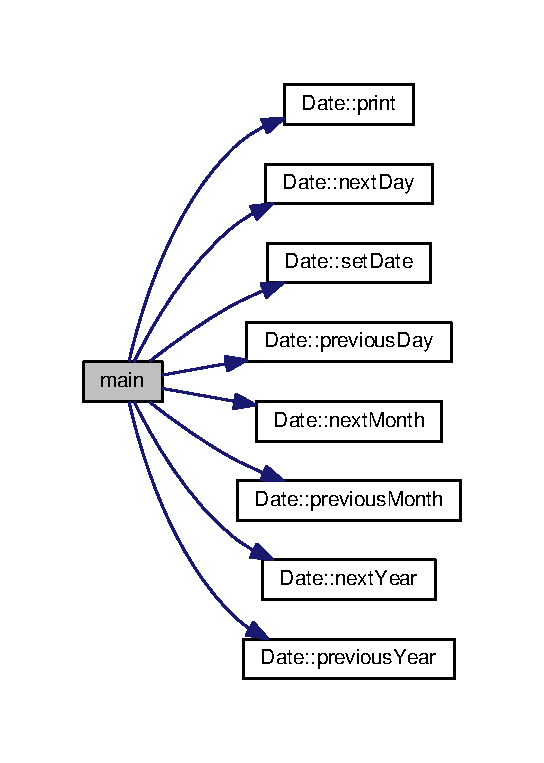
\includegraphics[width=261pt]{Dmain_8cpp_ae66f6b31b5ad750f1fe042a706a4e3d4_cgraph}
\end{center}
\end{figure}



%--- End generated contents ---

% Index
\backmatter
\newpage
\phantomsection
\clearemptydoublepage
\addcontentsline{toc}{chapter}{Index}
\printindex

\end{document}
